\documentclass[12pt,a5paper]{book}
\usepackage[utf8]{vietnam}
\usepackage{amsmath}
\usepackage{verbatim}
\usepackage{amsfonts}
\usepackage{tikz}
\usetikzlibrary{arrows,automata,shapes.geometric}
\usepackage{amssymb}
\usepackage{graphicx}
\usepackage{listings}
\usepackage{textcomp}
\usepackage[hidelinks]{hyperref}

\renewcommand{\familydefault}{\sfdefault}
\usepackage[left=2cm,right=1.5cm,top=1.5cm,bottom=1.5cm]{geometry}

 \renewcommand\lstlistingname{Quelltext} % Change language of section name

\lstset{ % General setup for the package
	language=C,
	basicstyle=\small\sffamily,
	numbers=left,
 	numberstyle=\tiny,
	frame=tb,
	tabsize=4,
	columns=fixed,
	showstringspaces=false,
	showtabs=false,
	keepspaces,
	%commentstyle=\color{green},
	%keywordstyle=\color{blue}
}
\tikzstyle{startstop} = [rectangle, rounded corners, minimum width=2cm, minimum height=0.25,text centered, draw=black]
\tikzstyle{io} = [trapezium, trapezium left angle=70, trapezium right angle=110, minimum width=3cm, minimum height=1cm, text centered, draw=black]
\tikzstyle{process} = [rectangle, minimum width=2cm, minimum height=0.25, text centered, draw=black]
\tikzstyle{decision} = [diamond, minimum width=2cm, minimum height=0.25, text centered, draw=black]
\tikzstyle{arrow} = [thick,->,>=stealth]
\pagenumbering{gobble}
\pagenumbering{arabic}
\title{LẬP TRÌNH NHÚNG: chuyện chưa kể}
\author{Nguyễn Thành Công}


\begin{document}
\maketitle
\begin{figure}
\centering
 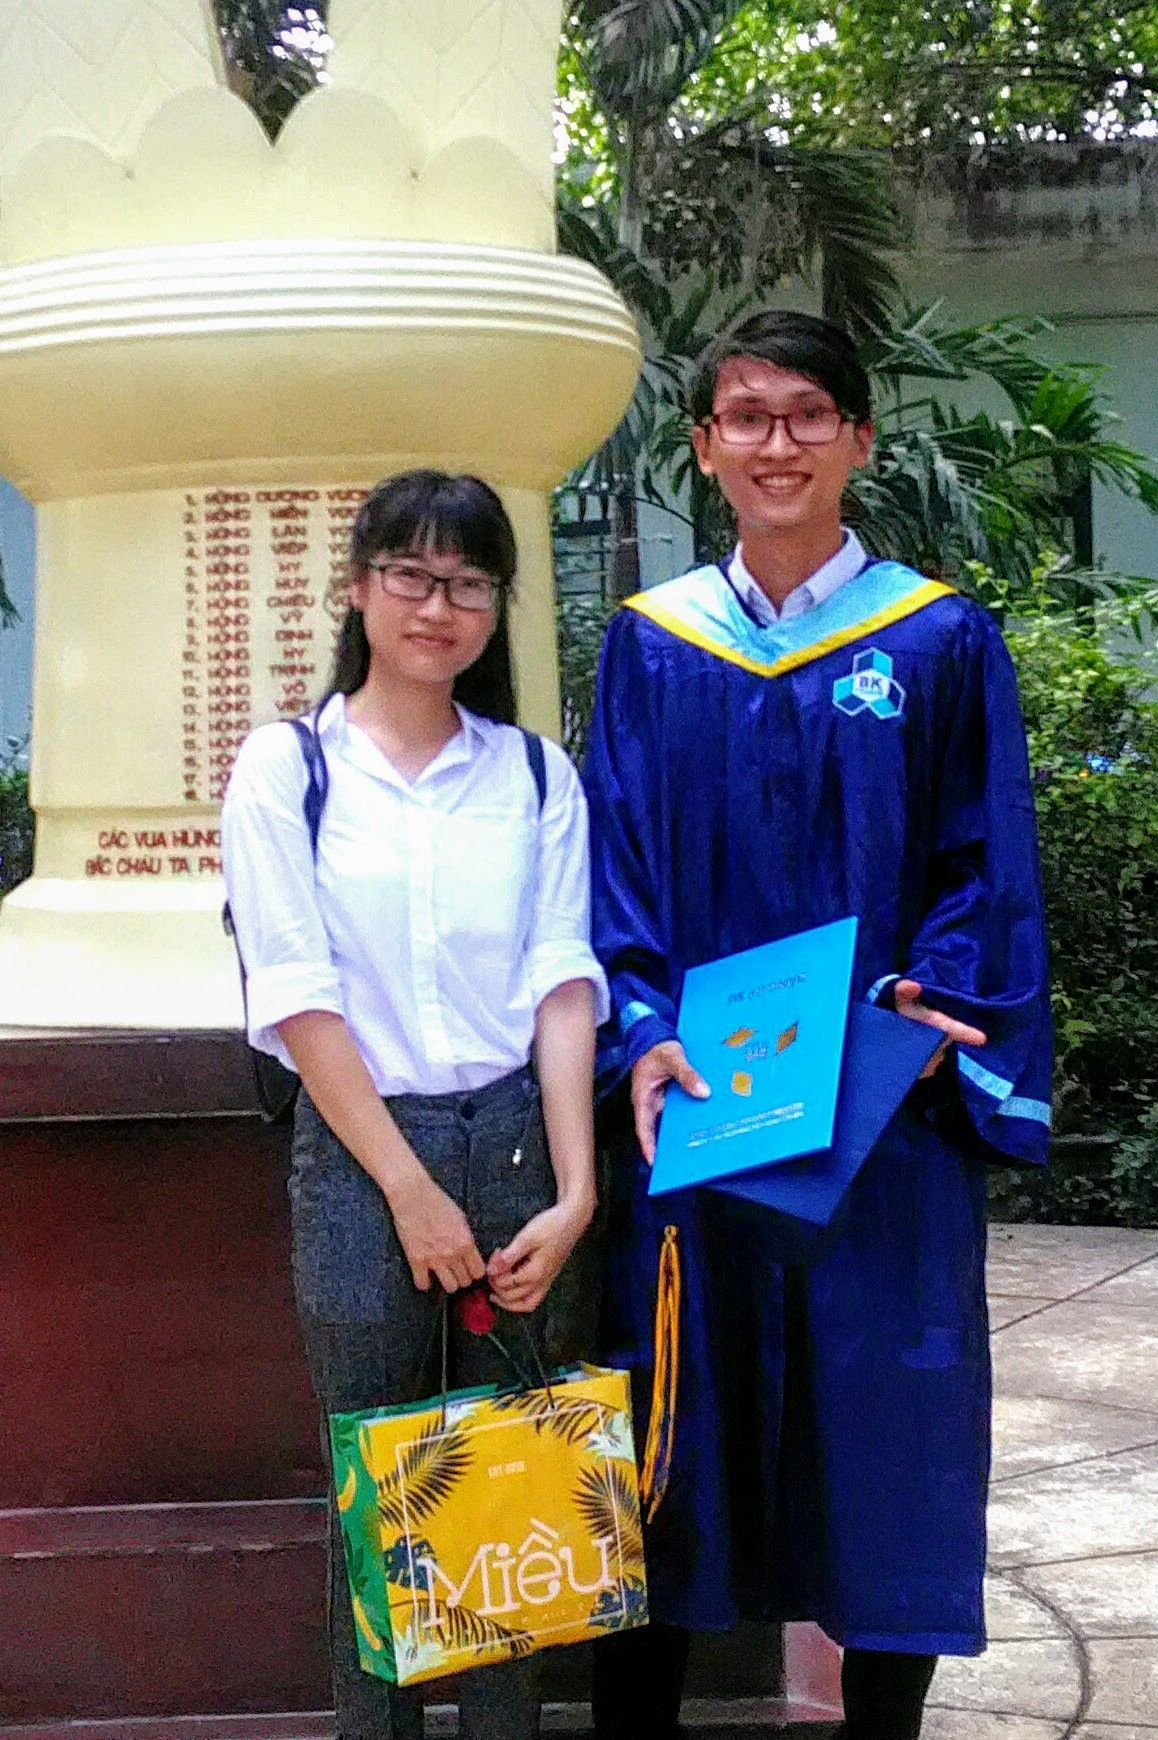
\includegraphics[width=0.5\linewidth]{tao.jpg}
 \caption{Tui}
\end{figure}
\tableofcontents{}
 \chapter{Chém gió xíu }
	\section{Về lập trình nhúng}
		\paragraph{}
Đặc trưng của lập trình nhúng là viết chương trình để điều khiển phần cứng, ví dụ như chương trình điều khiển động cơ bước chẳng hạn. Với phần mềm ứng dụng như trên máy tính mà phần cứng yêu cầu giống nhau (màn hình, chuột, cpu...) và đòi hỏi nặng về khả năng tính toán của cpu. Còn với chương trình nhúng thì phần cứng của nó cực kì đa dạng, khác nhau với mỗi ứng dụng như chương trình điều khiển động cơ hoặc chương trình đọc cảm biến, nó không đòi hỏi cpu phải tính toán quá nhiều, chỉ cần quản lý tốt phần cứng bên dưới. 
		\paragraph{}
Có 2 khái niệm là Firmware, ý chỉ chương trình nhúng, và Software, chương trình ứng dụng trên máy tính, được đưa ra để người lập trình dễ hình dung, nhưng không cần thiết phải phân biệt rõ ràng.
		\paragraph{}
Khi lập trình hệ thống nhúng, việc biết rõ về phần cứng là điều cần thiết. Bởi bạn phải biết phần cứng của mình như thế nào thì bạn mới điều khiển hoặc quản lí tốt nó được. Tốt nhất là làm trong team hardware một thời gian rồi nhảy qua team firmware, hoặc làm song song cả hai bên (nếu bạn đủ sức).
		\paragraph{}
Tóm lại: \textit{Lập trình nhúng là viết chương trình điều khiển phần cứng, bạn phải biết lập trình, và phải giỏi về phần cứng.} 
	\section{Về ngôn ngữ C trong lập trình nhúng}
		\paragraph{}
	Ngôn ngữ C cho phép tương tác rất mạnh tới phần cứng, mạnh thế nào thì hồi sau sẽ rõ, thế nên nó thường được lựa chọn trong các dự án lâp trình nhúng. Ngoài ra có thể dùng C++ và Java nhưng mình ít xài chúng nên không đề cập ở đây.
		\paragraph{}
	Việc học C cơ bản mình sẽ không đề cập tới vì tài liệu nó nhiều lắm, các bạn có để xem và làm vài bài tập sử dụng được ngôn ngữ này. Lưu ý là ranh giới giữa việc \textbf{biết} và \textbf{sử dụng được} ngôn ngữ C là việc bạn có làm bài tập hay không. Về cú pháp thì nó quanh đi quẩn lại chỉ là khai báo biến, rồi mấy vòng lặp for, while hoặc rẽ nhánh if, else chẳng hạn, nhưng \textbf{kỹ năng} sử dụng C để giải quyết một vấn đề thì cần nhiều bài tập để trau dồi.
		\paragraph{}
	Tóm lại: \textit{bạn không thể đọc sách học bơi là biết bơi, không thể đọc kiếm phổ là thành cao thủ.}
	\section{Về phần cứng để demo}
	\paragraph{}
	Trong phần này mình sẽ sử dụng 2 con Arduino Mega để demo cho nhanh. Bạn nên mua để dành nháp một vài cái project nào đấy. Mà thiệt tình thì nên hạn chế sử dụng Arduino vì nó làm bạn có thói quen sử dụng thư viện chùa với lại chẳng biết gì mấy về phần cứng, đến lúc Arduino chưa có thư viện thì không biết phải viết thế nào. Bạn có thể tìm hiểu các loại chip khác như STM32 (nó rất mạnh trong tầm giá của nó), PIC(nó bền và ổn định) hay xài kit Tiva cũng được. Ngoài ra phần thiên về lập trình không cần phần cứng sẽ sử dụng chương trình DevC++ (nhớ tạo project C, không cần C++), những cái cơ bản các bạn nên tự tìm hiểu, vì những cái đó tài liệu nó rất nhiều, và bạn cũng có thể tự mò cho quen.
	\paragraph{}
	\textit{Arduino là món mì ăn liền, sử dụng nó nhanh chóng nhưng nó cũng đầy điểm yếu.}
	\section{Về Tiếng Anh, vâng tiếng Anh...}
		\paragraph{}
	Mấy ngành khác thì mình không rành chứ mà làm nhúng mà bạn không biết Tiếng Anh là tự níu chân mình lại. Vì mỗi linh kiện điện tử đều kèm theo một cái bảng thông tin đặc tính là datasheet, cái nào phức tạp thì sẽ kèm theo một cái hướng dẫn sử dụng là user manual. Và tất nhiên 96.69\% chúng được viết bằng tiếng Anh, còn lại là tiếng Trung Quốc. Và tin buồn là code trong lập trình nhúng đều biết bằng tiếng Anh, tin buồn hơn nữa là tài liệu, sách hướng dẫn, các diễn đàn sử dụng tiếng Anh rất nhiều và nhiều cái rất hay.
		\paragraph{}
	Tóm lại là không biết nó thì công việc của bạn bị cản trở rất nhiều, phụ thuộc rất nhiều vào google dịch củ chuối. Hãy dừng một bước để học tiếng anh và tiến 3 bước trong con đường sự nghiệp. Chí ít bạn phải đọc được datasheet mà không cần tra quá nhiều từ, đọc được cuốn sách như clean code chẳng hạn, hoặc viết email cho thằng bán linh kiện ở Trung Quốc vì kiểu gì sau này bạn cũng đặt hàng ở bên đó.
		\paragraph{}
	\textit{Nhớ rằng tiếng Anh là công cụ để sử dụng. Như người ta học đi xe máy để đi lại nhanh hơn. Hãy học tiếng Anh để làm việc ngon lành hơn.}


	\chapter{Ngôn ngữ C trong lập trình nhúng}
	\paragraph{}
Hãy nhớ là bạn làm vài bài tập về ngôn ngữ C rồi hãy đọc phần này nhé!!!. Có mấy cuốn sách mà mình để ở mục tham khảo, bạn cũng nên xem coi mặt mũi tụi nó thế nào.
	\section{Cơ bản về chương trình.}
	\paragraph{} 
Đại khái thì việc lập trình là chỉ cho cái máy biết bạn muốn nó làm cái gì.
	\paragraph{}
Khi bạn viết chương trình, bên dịch thì máy tính sẽ biên dịch code của bạn (người hiểu được) thành mã máy (máy hiểu được) bao gồm các lệnh mà vi điều khiển sẽ thực và khi nạp xuống cho vi điều khiển thì chương trình sẽ được lưu ở ROM (bộ nhớ chương trình). CPU sẽ đọc lệnh từ bộ nhớ chương trình rồi thực thi. Lưu ý là CPU chỉ đọc thôi, nó không được phép ghi gì vào bộ nhớ chương trình. Nó không thể cãi lệnh bạn! Thế nên bộ nhớ chương trình có tên là bộ nhớ chỉ đọc (Read-only memory, ROM). Nó vẫn còn đấy khi mất điện.
	\paragraph{}
Còn bộ nhớ RAM là để phục vụ cho chương trình được thực thi.
	\paragraph{}
Ví dụ như bạn khai báo biến int a=0; thì biến a sẽ được lưu trong RAM. Sau đó có lệnh a=a+1; CPU sẽ lấy biến a từ trong RAM ra, thực hiện phép tính rồi lại lưu vào chỗ cũ.
	\paragraph{}
Do việc RAM được CPU sử dụng để thực hiện chương trình, đọc ghi liên tục nên nó gọi là bộ nhớ truy cập ngẫu nhiên (Random-access Memory) CPU đươc toàn quyền sử dụng bộ nhớ này. Khi mất điện thì chương trình phải chạy lại từ đầu nên những gì được lưu trong làm là không cần thiết và bị xóa trắng. Có một số chip có một vùng RAM nhỏ được nuôi bằng pin để lưu một vài thông số quan trọng, khi có điện lại thì chương trình đọc các thông số đó ra và chạy tiếp. Ví dụ như một dây chuyền sản xuất, nó phải lưu lại vị trí của dây chuyền để khi có điện lại thì nó chạy luôn được ngay.

	\section{Về cách tổ chức bộ nhớ}
	\paragraph{}
	Thông thường thì đơn vị nhỏ nhất của bộ nhớ là byte (mà mình hay gọi là ô nhớ), mỗi byte đươc đánh một địa chỉ. Tùy số lượng bit của bus địa chỉ mà quyết định xem nó có thể quản lý bao nhiêu ô nhớ. Nếu bus địa chỉ 8-bit thì nó có thể quản lý 256 byte bộ nhớ, bus địa chỉ 16-bit thì có thể quản lý 64kbyte, còn 32-bit thì có thể quản lý tới 4Gbyte bộ nhớ. 
	
\begin{figure}[h!]
	\centering
	
	%\label{fig:Bộ nhớ 16 bit}
	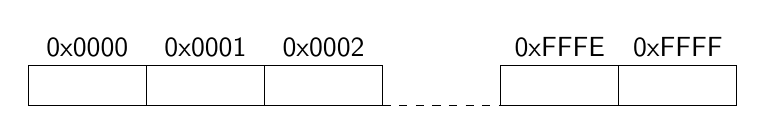
\begin{tikzpicture}[yscale=0.5, xscale=1.5]

		\draw (0,0) rectangle (1,1);
		\draw (1,0) rectangle (2,1);
		\draw (2,0) rectangle (3,1);
		\draw [dashed] (3,0) -- (4,0);
		\draw (4,0) rectangle (5,1);
		\draw (5,0) rectangle (6,1);
		\node  [above] at (0.5, 1) {0x0000};
		\node  [above] at (1.5, 1) {0x0001};
		\node  [above] at (2.5, 1) {0x0002};
		\node  [above] at (4.5, 1) {0xFFFE};
		\node  [above] at (5.5, 1) {0xFFFF};
	\end{tikzpicture}
	\caption{Bộ nhớ địa chỉ 16-bit} 
\end{figure}

	Vậy mỗi ô nhớ sẽ có 2 thông số mà bạn cần quan tâm: địa chỉ (nó ở đâu, địa chỉ có thể là số 8-bit, 16-bit, 32-bit...), và giá trị được lưu (nó bao nhiêu, chỉ là số 8-bit (1 byte) thôi).
	
	\begin{figure}[h!]
	\centering
	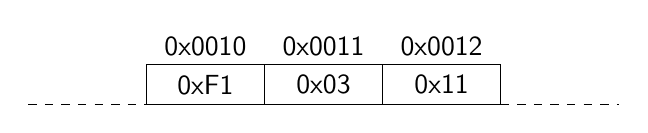
\begin{tikzpicture}[yscale=0.5, xscale=1.5]
		\draw [dashed] (0,0) -- (1,0);
		\draw (1,0) rectangle (2,1);
		\draw (2,0) rectangle (3,1);
		\draw (3,0) rectangle (4,1);
		\draw [dashed] (4,0) -- (5,0);
		
		\node  [above] at (1.5, 1) {0x0010};
		\node  [above] at (2.5, 1) {0x0011};
		\node  [above] at (3.5, 1) {0x0012};
		\node   at (1.5, 0.5) {0xF1};
		\node   at (2.5, 0.5) {0x03};
		\node   at (3.5, 0.5) {0x11};

	\end{tikzpicture}
	\caption{Dữ liệu trong bộ nhớ} %\label{fig: Dữ liệu trong bộ nhớ}
\end{figure}

	\paragraph{}

	Đoạn chương trình để xem địa chỉ trong DevC++:\*
\begin{lstlisting}
	#include <stdio.h>
	void main(){
		char a;
		printf("a address: 0x%08x\n", &a);
	}
\end{lstlisting}

	
	\section{Khai báo biến}
	\paragraph{}
Các kiểu biến thông thường khi lập trình C là char, int, long, float double. Nhưng trong lập trình nhúng, tài nguyên bộ nhớ hạn chế nên việc bạn biết các biến chiếm bao nhiêu ô nhớ là điều rất quan trọng. Thông thường, các biến được khai báo dưới dạng uint8\_t, int8\_t, uint16\_t, int16\_t... để sử dụng thì bạn cần  \#include <stdint.h>. Đoán xem mỗi kiểu sẽ chiếm bao nhiêu ô nhớ, và kiểu nào là kiểu có dấu, không đấu?
	\paragraph{}
	Một điểm đặc biệt là kiểu uint8\_t thường được dùng để đại diện cho một ô nhớ (8-bit). Ví dụ khi khai báo uint8\_t array[3], thì có thể hiểu là khai báo 3 phần tử mảng array có kiểu là uint8\_t, hoặc cũng có thể hiểu là yêu cầu bộ nhớ cấp 3 ô nhớ kề nhau. Việc này thường được dùng để khai báo các bộ đệm trong các giao tiếp như uart, i2c, spi...
	\paragraph{}
	Thế nên hãy thường sử dụng các kiểu dữ liệu với bộ nhớ tường minh trên để kiểm soát bộ nhớ chặt chẽ hơn.\\
\section{Kiểu dữ liệu tự định nghĩa}
\paragraph{}
Ngôn ngữ C cung cấp cơ chế tự định nghĩa kiểu dữ liệu để việc truy xuất dữ liệu được thuận tiện.

\paragraph{}
Ví dụ mình có một cái cảm biến có thể đọc về nhiệt độ, độ ẩm và ánh sáng môi trường. Dữ liệu nhiệt độ từ  -20\textdegree{}C đến 100\textdegree{}C, độ ẩm từ 0\% đến 100\%, ánh sáng từ 0 lux đến 50.000 lux. Vậy mình khai báo dữ kiểu dữ liệu env\_t (environment type) như sau: 
\begin{lstlisting}
	typedef struct{
		int8_t temp;
		uint8_t humi;
		uint16_t lux;
	}env_t;
\end{lstlisting}
\paragraph{}
Dễ thấy là các kiểu biến bên trong đều chứa đủ khoảng giá trị cần thiết (nếu nhiệt độ vượt quá 127\textdegree{}C thì biến int8\_t không chứa được, phải chọn kiểu khác).
\paragraph{}
Thực chất kiểu dữ liệu là cách bạn tương tác với một vùng nhớ cho trước. Ví dụ khi khai báo một biến như \textit{env\_t evn;} chẳng hạn, nó sẽ cung cấp cho bạn 4 ô nhớ liền nhau. Nếu bạn in địa chỉ của biến env ra nó sẽ hiển thị địa chỉ ô nhớ \textbf{đầu tiên} của dãy 4 ô nhớ đó. Và kiểu env\_t sẽ cho máy tính biết cách truy cập tới 4 ô nhớ đó như thế nào.

\begin{figure}[h!]
	\centering
	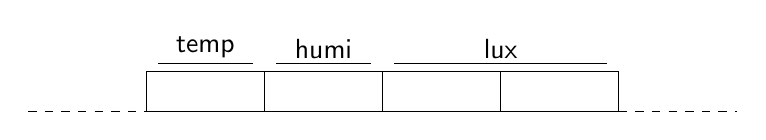
\begin{tikzpicture}[yscale=0.5, xscale=1.5]
		\draw [dashed] (0,0) -- (1,0);
		\draw (1,0) rectangle (2,1);
		\draw (2,0) rectangle (3,1);
		\draw (3,0) rectangle (4,1);
		\draw (4,0) rectangle (5,1);
		\draw [dashed] (5,0) -- (6,0);
		
		\draw (1.1, 1.2) -- (1.9, 1.2);
		\node [above] at (1.5, 1.1) {temp};
		
		\draw (2.1, 1.2) -- (2.9, 1.2);
		\node [above] at (2.5, 1.1) {humi};
		
		\draw (3.1, 1.2) -- (4.9, 1.2);
		\node [above] at (4, 1.1) {lux};
		
	\end{tikzpicture}
	\caption{Truy cập biến kiểu env\_t} %\label{fig: Dữ liệu trong bộ nhớ}
\end{figure}
\paragraph{}
Đoạn chương trình xem độ dài của kiểu dữ liệu:
\begin{lstlisting}
#include <stdio.h>
#include <stdint.h>

typedef struct{
	int8_t temp;
	uint8_t humi;
	uint16_t lux;
}env_t;

void main(void) {
	printf("Size of env_t: %d\n", sizeof(env_t));
}
\end{lstlisting}
\paragraph{}
Một điểm cần lưu ý là các máy tính thường có cơ chế làm tròn biên kiểu dữ liệu (data structure alignment). Nếu chúng ta khai báo như sau:

\begin{lstlisting}
typedef struct{
	int8_t temp;
	uint16_t lux;
	uint8_t humi;
}env_t;
\end{lstlisting}
biến lux khai báo ở giữa, thì kiểu dữ liệu env\_t giờ đây có độ dài là 6 byte chứ không phải 4!!!.
\paragraph{}
Kiểu biến env\_t giờ có cấu trúc như sau:
\begin{figure}[h!]
	\centering
	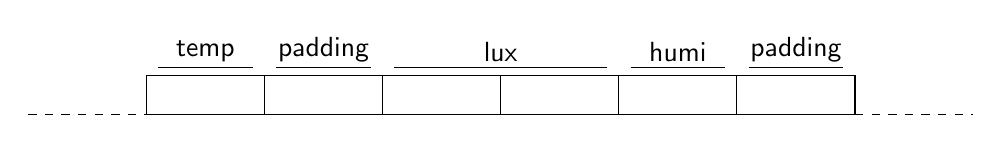
\begin{tikzpicture}[yscale=0.5, xscale=1.5]
		\draw [dashed] (0,0) -- (1,0);
		\draw (1,0) rectangle (2,1);
		\draw (2,0) rectangle (3,1);
		\draw (3,0) rectangle (4,1);
		\draw (4,0) rectangle (5,1);
		\draw (5,0) rectangle (6,1);
		\draw (6,0) rectangle (7,1);
		\draw [dashed] (7,0) -- (8,0);
		
		\draw (1.1, 1.2) -- (1.9, 1.2);
		\node [above] at (1.5, 1.1) {temp};
		
		\draw (2.1, 1.2) -- (2.9, 1.2);
		\node [above] at (2.5, 1.1) {padding};
		
		\draw (3.1, 1.2) -- (4.9, 1.2);
		\node [above] at (4, 1.1) {lux};
		
		\draw (5.1, 1.2) -- (5.9, 1.2);
		\node [above] at (5.5, 1.1) {humi};
		
		\draw (6.1, 1.2) -- (6.9, 1.2);
		\node [above] at (6.5, 1.1) {padding};
	\end{tikzpicture}
	\caption{Truy cập biến kiểu env\_t} 
\end{figure}
\paragraph{}
Hai ô nhớ tên padding được thêm vào để tăng hiệu suất việc đọc ghi dữ liệu trong máy tính hiện đại. Các bạn quan tâm thì có thể tìm hiểu thêm. Ta có thể tránh nó bằng cách khai báo như sau: trong DevC++ thì bạn khai báo \textit{\#pragma pack(1)} trước khi khai báo biến dữ liệu, còn trong nếu sử dụng KeilC cho chip STM32 hoặc kit Tiva thì khai báo kiểu:

\begin{lstlisting}
typedef __packed struct{
	int8_t temp;
	uint16_t lux;
	uint8_t humi;
}env_t;
\end{lstlisting}
mỗi khi khai báo một kiểu biến nào đó. Trong Arduino thì mình không thấy nó có cơ chế này.

\paragraph{}
Ngoài ra còn một số kiểu enum và union mà các bạn hỏi giáo sư gu gồ hen.

\section{Con trỏ}
\paragraph{}
Có thể nói con trỏ là công cụ lợi hại nhất của C, bạn khó mà giỏi C nếu bỏ qua con trỏ được. Bản chất của con trỏ (chưa nói đến con trỏ hàm) là trỏ tới một vùng nhớ nào đó và tương tác với vùng nhớ đó. Chương trình ví dụ về con trỏ:
\begin{lstlisting}
#include <stdio.h>
#include <stdint.h>

int main(void) {
	uint16_t a=0;
	uint16_t *pa;
	pa=&a;
	printf("a addr: 0x%08x\n", &a);
	printf("a addr: 0x%08x\n", pa);
}
\end{lstlisting}

hai lần printf sẽ cho ra kết quả như nhau vì đã gán địa chỉ của a cho pa.
\paragraph{}
Lưu ý là bạn không cần quan tâm địa chỉ thật của a (có dạng số hex như 0x0012) chỉ cần khai báo biến a, nó sẽ nằm đâu đó trong RAM (nếu RAM còn trống) và có phép lấy địa chỉ \&a.
\paragraph{}
Một con trỏ cần 2 thông tin sau để có thể hoạt động được: \textbf{địa chỉ} và \textbf{kiểu dữ liệu} nó sẽ trỏ tới. Như chương trình trên thì dòng số 6 sẽ cấp cho con trỏ kiểu dữ liệu, dòng số 7 cấp địa chỉ. 2 yếu tố trên giúp bạn có thể đi đến vùng nhớ mà bạn quan tâm sau đó có thể truy cập vùng nhớ đó theo cách bạn muốn.
\paragraph{}
Một lưu ý là ngôn ngữ C đồng nhất giữa mảng và con trỏ. Ví dụ mình khai báo mảng uint32\_t arr[4], thì \textit{arr} là địa chỉ của phần tử đầu tiên của mảng, hay arr=\&arr[0] (cùng 1 địa chỉ), *arr=arr[0] (cùng 1 giá trị). Giả sử arr là địa chỉ 0x0010 thì arr+1 sẽ là địa chỉ của arr[1] có địa chỉ là 0x0014 (không phải 0x0011 he, đo mỗi biến có 4 ô nhớ, kiểm tra lại bằng DevC++).
\section{Ví dụ về truyền nhận uart}

\paragraph{}
Để biết con trỏ nó lợi hại như thế nào thì các bạn hãy xem ví dụ về truyền nhận uart.
\paragraph{}
Các hàm truyền nhận dữ liệu uart thường có cấu trúc như sau:
\begin{lstlisting}
uart_transmit(uint8_t *data, uint16_t size);
uart_receive(uint8_t *data, uint16_t size);
\end{lstlisting}
\paragraph{}
Trong hàm uart\_transmit, tham số *data là ô nhớ đầu tiên trong chuỗi ô nhớ liên tiếp mà bạn muốn gửi đi. Còn trong hàm uart\_receive, tham số *data là ô nhớ đầu tiên của vùng nhớ mà bạn sẽ cất dữ liệu nhận được vào đấy (địa chỉ bộ đệm).
\subsection{Truyền uart}
\paragraph{}
Mình ví dụ chương trình sau: một MCU đọc cảm biến môi trường, lưu vào biến env (khai báo ở trên), rồi truyền qua đường uart về một MCU khác để xử lý.

\paragraph{}
Vậy giờ mình cần gửi một biến env (khi đã nhập dữ liệu cho biến này) đi thì cần làm thế nào để hàm truyền kia có thể truyền một kiểu env\_t đi trong khi hàm truyền nhận uart chỉ nhận vào là kiểu uint8\_t?
\paragraph{}
Cách giải quyết của mình là thế này, tạo một con trỏ kiểu uint8\_t và cấp cho nó địa chỉ của biến env.
\begin{lstlisting}
env_t evn; //env.temp=10; env.humi=70, env.lux=1000;
uint8_t *pe;
pe=(uint8_t *)&evn;
uart_transmit(pe, sizeof(env_t));
\end{lstlisting}
\paragraph{}
Câu lệnh dòng số 3, \textit{pe=(uint8\_t *)\&evn} có 2 phần: đầu tiên là \&evn, lấy địa chỉ của biến env tạo thành một con trỏ tạm thời kiểu evn\_t, sau đó ép kiểu con trỏ (uint8\_t *) và gán cho pe. Vậy pe là một con trỏ kiểu uint8\_t và có địa chỉ của biến env, sau đó mình dùng hàm uart truyền đi 4 ô nhớ bắt đầu từ ô nhớ này. Mấy bạn chưa quen thì nên ngâm cứu kĩ chỗ này :)))
\paragraph{}
Khi sử dụng đến con trỏ, bạn cần có \textbf{tư duy ở ô nhớ} (chứ không phải kiểu dữ liệu) thì việc sử dụng con trỏ sẽ đơn giản hơn rất nhiều. Ví dụ như trong hàm truyền uart, với kiểu uint8\_t đại diện cho ô nhớ, và hai tham số *data và size, có ý nói là hãy đưa tôi địa chỉ ô nhớ đầu tiên và số lượng cần truyền, tôi sẽ truyền cái đống đó đi cho bạn.
\subsection{Nhận uart}
\paragraph{}
Phía nhận muốn nhận được dữ liệu thì trước tiên phải khai báo một bộ đệm, sau đó gọi hàm uart\_receive() trỏ tới bộ đệm này và chờ dữ liệu đến.
\begin{lstlisting}
#define MAX_BUFF 10
uint8_t uart_buffer[MAX_BUFF];
uart_receive(uart_buffer, sizeof(env_t));
\end{lstlisting}
\paragraph{}
Lưu ý là số lượng ô nhớ của bộ đệm phải lớn hớn hoặc bằng số lượng trong một lần truyền, nếu không chương trình sẽ lỗi. Câu lệnh số 1 để định nghĩa số lượng và để lên trên cùng của trang để sau này sửa lại số lượng cho phù hợp (cỡ như chương trình của bạn 1000 dòng mà nhét thẳng số 10 vô khai báo mảng luôn mai mốt tìm lại đuối).
\paragraph{}
Rồi, sau khi nhận được dữ liệu, việc của bạn là đọc dữ liệu và hiển thị lên màn hình lcd hoặc cất đâu đó. Ta tiến hành ép kiểu một lần nữa
\begin{lstlisting}
env_t *p_env;
p_env = (env_t *)uart_buffer;

\end{lstlisting}
để có được con trỏ kiểu env\_t và trỏ đến vùng nhớ ta vừa nhận được. Sau đó ta có thể sử dụng con trỏ này.
\begin{lstlisting}
printf("Temperature: %d\n", p_env->temp);
printf("Humidity: %d\n", p_env->humi);
printf("Lux: %d\n", p_env->lux);

\end{lstlisting}
\paragraph{}
Như vậy là cùng nhiêu đó ô nhớ nhưng \textbf{cách nhìn các ô nhớ đó} khác nhau với những kiểu dữ liệu khác nhau. Việc ép kiểu không làm thay đổi nội dung của ô nhớ vật lý (nó vẫn là cái đống 00 11 đó thôi), nhưng nó thay đổi cách bạn đọc nó.
\begin{figure}[h!]
	\centering
	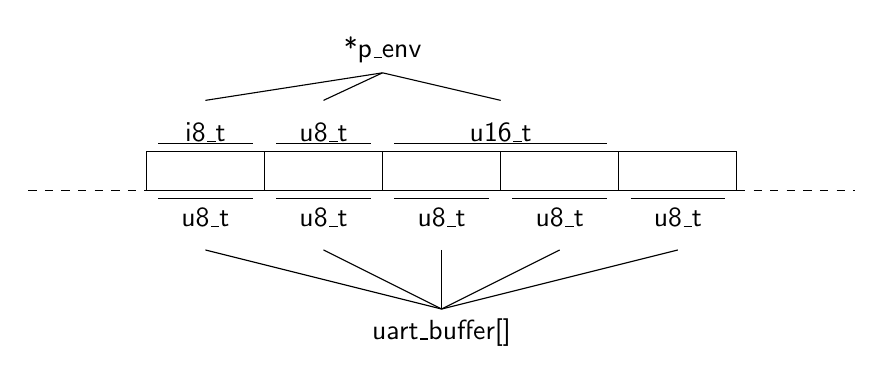
\begin{tikzpicture}[yscale=0.5, xscale=1.5]
		\draw [dashed] (0,0) -- (1,0);
		\draw (1,0) rectangle (2,1);
		\draw (2,0) rectangle (3,1);
		\draw (3,0) rectangle (4,1);
		\draw (4,0) rectangle (5,1);
		\draw (5,0) rectangle (6,1);
		\draw [dashed] (6,0) -- (7,0);
		
		\draw (1.1, 1.2) -- (1.9, 1.2);
		\node [above] at (1.5, 1) {i8\_t};
		\draw (1.5,2.3)--(3,3);		
		
		\draw (2.1, 1.2) -- (2.9, 1.2);
		\node [above] at (2.5, 1) {u8\_t};
		\draw (2.5,2.3)--(3,3);		
		
		\draw (3.1, 1.2) -- (4.9, 1.2);
		\node [above] at (4, 1) {u16\_t};
		\draw (4,2.3)--(3,3);	
		
		\node [above] at (3, 3) {*p\_env};
		
		\draw (1.1, -0.2) --(1.9,-0.2);
		\node [below] at (1.5, -0.2) {u8\_t};
		\draw (1.5, -1.5) -- (3.5,-3);

		\draw (2.1, -0.2) --(2.9,-0.2);
		\node [below] at (2.5, -0.2) {u8\_t};
		\draw (2.5, -1.5) -- (3.5,-3);

		\draw (3.1, -0.2) --(3.9,-0.2);
		\node [below] at (3.5, -0.2) {u8\_t};
		\draw (3.5, -1.5) -- (3.5,-3);

		\draw (4.1, -0.2) --(4.9,-0.2);
		\node [below] at (4.5, -0.2) {u8\_t};
		\draw (4.5, -1.5) -- (3.5,-3);

		\draw (5.1, -0.2) --(5.9,-0.2);
		\node [below] at (5.5, -0.2) {u8\_t};
		\draw (5.5, -1.5) -- (3.5,-3);
		
		\node [below] at (3.5, -3) {uart\_buffer[]};
		
	\end{tikzpicture}
	\caption{Buffer v.s env\_t.}
\end{figure}
\paragraph{}
Rồi đến đây các bạn có thể cảm nhận được sức mạnh của con trỏ rồi, bạn có thể \textbf{chạm} đến bất cứ vùng nhớ nào và truy xuất theo \textbf{kiểu} mà bạn muốn. Thiệc là dễ quá chừng :))
\paragraph{}
Có một cách hiểu khác thế này, mỗi khi khai báo một con trỏ với một kiểu dữ liệu nào đấy, bạn đang khai báo một cái mặt nạ, hay một cái cách để khai thác dữ liệu.
\begin{figure}[h!]
	\centering
	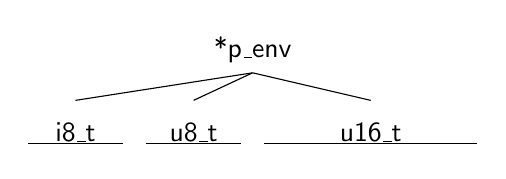
\begin{tikzpicture}[yscale=0.5, xscale=1.5]

		\draw (1.1, 1.2) -- (1.9, 1.2);
		\node [above] at (1.5, 1) {i8\_t};
		\draw (1.5,2.3)--(3,3);		
		
		\draw (2.1, 1.2) -- (2.9, 1.2);
		\node [above] at (2.5, 1) {u8\_t};
		\draw (2.5,2.3)--(3,3);		
		
		\draw (3.1, 1.2) -- (4.9, 1.2);
		\node [above] at (4, 1) {u16\_t};
		\draw (4,2.3)--(3,3);	
		
		\node [above] at (3, 3) {*p\_env};

	\end{tikzpicture}
	\caption{The mask}
\end{figure}
\paragraph{}
Bạn chưa thể đọc được dữ liệu nào cả vì mới chỉ khai báo cái cách truy cập dữ liệu thôi. Còn khi cấp địa chỉ cho con trỏ thì bạn đang ráp cái mặt nạ đó vào một hàng ô nhớ liên tục và sau có thể truy cập các ô nhớ đó theo cách này (hình 2.7).

\begin{figure}[h!]
	\centering
	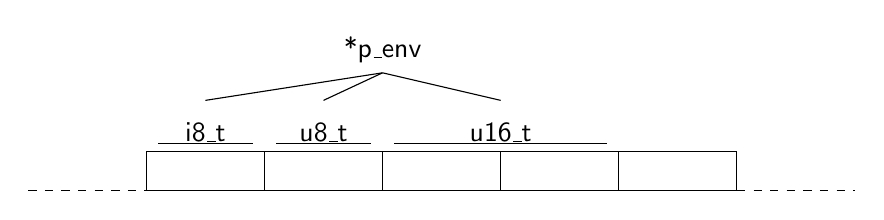
\begin{tikzpicture}[yscale=0.5, xscale=1.5]
		\draw [dashed] (0,0) -- (1,0);
		\draw (1,0) rectangle (2,1);
		\draw (2,0) rectangle (3,1);
		\draw (3,0) rectangle (4,1);
		\draw (4,0) rectangle (5,1);
		\draw (5,0) rectangle (6,1);
		\draw [dashed] (6,0) -- (7,0);
		
		\draw (1.1, 1.2) -- (1.9, 1.2);
		\node [above] at (1.5, 1) {i8\_t};
		\draw (1.5,2.3)--(3,3);		
		
		\draw (2.1, 1.2) -- (2.9, 1.2);
		\node [above] at (2.5, 1) {u8\_t};
		\draw (2.5,2.3)--(3,3);		
		
		\draw (3.1, 1.2) -- (4.9, 1.2);
		\node [above] at (4, 1) {u16\_t};
		\draw (4,2.3)--(3,3);	
		
		\node [above] at (3, 3) {*p\_env};
		
	\end{tikzpicture}
	\caption{The mask and the data.}
\end{figure}
\newpage
\paragraph{}
Lưu ý: bộ đêm là nơi dữ liệu đến và đi liên tục, nó là bến đỗ chứ không phải là chỗ chứa dữ liệu. Dữ liệu mới ập đến có thể ghi đè lên dữ liệu cũ. Nên cất vào đâu đấy rồi hãy xử lý gì đó tiếp theo
\begin{lstlisting}
env_t *p_env;
p_env = (env_t *)uart_buffer;
env_t recv_env=*p_env;
printf("Temperature: %d\n",  recv_env.temp);
printf("Humidity: %d\n",  recv_env.humi);
printf("Lux: %d\n",  recv_env.lux);
\end{lstlisting}
và việc ép kiểu này chỉ đúng nếu hai bên gửi và nhận có cùng cơ chế bộ nhớ hoặc big-endian hoặc little-endian thôi. Nếu khác kiểu thì không sử dụng được.
\section{Debug}
\paragraph{}
Khi viết một chương trình thì nhất thiết phải có công cụ để theo dõi coi code của bạn nó đang làm cái gì ở trỏng. Nếu ở lập trình C thuần túy bằng cái IDE như DevC++ hoặc Visual Studio thì bạn chỉ cần gọi hàm printf ra và in cái gì trong đó bạn muốn. Còn trong lập trình nhúng thì con MCU của bạn nó chạy chứ không phải CPU của máy tính. Muốn MCU in ra được những dòng chữ lên màn hình desktop thì cần theo quy trình sau: MCU truyền qua uart, qua một module chuyển uart-usb đã cắm vào máy tính, một chương trình đọc cổng COM trên máy tính và hiển thị chuỗi kí tự nhận được.
\paragraph{}
Trên board Arduino có sẵn bộ chuyển usb-uart rồi, thường là cổng uart 0 (Serial 0). Code để demo mình đã để sẵn trên \textit{\url{https://github.com/congkeodhbk/Lap_trinh_nhung}}. 
\paragraph{}
Có 2 board, một cái nạp chương trình transmit và một cái nạp receive. Chương trình transmit liên tục gửi biến về. Còn receive thì đọc và hiển thị kết quả. Tuy nhiên bên receive nó hơi phức tạp xíu. Giả sử mình nhận mà không biết thằng gửi sẽ gửi bao nhiêu byte thì sao? Vậy mình sẽ sử dụng cách đại khái là khi nó đang nhận mà không thấy dữ liệu đến nữa trong vòng 20 mili giây thì nó hiểu là đã nhận xong. Các bạn đọc code rồi mò coi cắm chân cẳng thế nào để cái đứa nói chuyện được với nhau. Và xa hơn bạn thử lấy môt cái chip khác, như stm32f4 chẳng hạn, viết chương trình tương tự code transmit và gửi cho Arduino receive nhận xem nó có chạy không. Và xa tới đầu hẻm nữa thì viết tất cả mọi thứ lên chip khác, cả thư viện debug của mình.
\paragraph{}
Trong thư viện trên mới chỉ có hàm debug() tương đương với printf() trong C, còn nhiều cách debug xịn hơn, như làm thế nào sử dụng lệnh tương tự scanf trong C lên board Arduino, bạn nhập lệnh trên màn hình console của máy tính và chuyển xuống Arduino, tùy mỗi lệnh bạn nhập mà nó chạy những kịch bản khác nhau.
\paragraph{}
\chapter{Coding style}
\paragraph{}
Coding style là gì? Nếu như bạn thấy code của bạn rối tung rối mù, lấy code của thằng bạn đọc để fix bug cho nó mà đọc muốn rớt con mắt ra ngoài, hay thêm một tính năng mới rồi okie, đập đi hết cái mớ bạn code rồi xây lại.
\paragraph{}
Và coding style giúp bạn giải quyết mấy chuyện đó, tuyệt vời!!! Và làm sao mà nó có thể làm được vậy?
\paragraph{}
Có 3 yêu cầu chính mà người lập trình cần đáp ứng cho chương trình: chạy được, dễ thay đổi, dễ hiểu.
\begin{itemize}
  \item Chạy được: Tất nhiên là mọi người đều hướng tới mục tiêu này, không chạy được thì có code cũng như không.
  \item Dễ thay đổi: yếu tố chạy được là đáp ứng được tiêu chí đề ra. Nhưng mà với lập trình thực tế thì các tiêu chí đó liêu tục bị thay đổi. Giống như việc ông sếp thấy phương án này chua ăn quá nên đổi qua cái kia, ông khách hàng thì muốn thêm tính năng này, đề xuất cái kia. Ví dụ như bạn đi, làm một cái xe nhỏ nhỏ dò line, làm xong rồi muốn gắn cái camera vô xử lý ảnh cho chạy, làm xong rồi nữa thì muốn gắn thêm đèn chớp chớp cho vui chẳng hạn. Hoặc mục tiêu bạn đâu thực hiện xong rồi mà thấy nó chạy chưa ngon, muốn viết lại xíu để nâng cấp firmware lên, giờ nhìn vô cái đống bùng nhùng kia hông lẽ đập đi xây lại?
	\item Dễ hiểu: vì các dự án thực tế đều cần làm nhóm cả. Bạn sử dụng code của người khác để viết thêm, người sau này sẽ dùng code của bạn thể phát triển, nâng cấp bảo trì chẳng hạn. Hoặc chính bạn sau một thời gian đọc lại code của mình có khi không biết ngày xưa mình vẽ bùa gì trong đây nữa. Nên code phải viết làm sao cho người khác có thể đọc được (tất nhiên thằng đó nó phải được được xíu, đừng có gà quá).
\end{itemize}
\paragraph{}
Có thể khẳng định thế này, lập trình không có khó, ngồi fix bug mới mệt. Thế nên việc có coding style sẽ làm cho cuộc sống của bạn dễ chịu hơn rất nhiều. Ngoài việc chịu khó ngồi code là còn phải đọc sách hoặc thỉnh giáo cách sư phụ để làm thế nào cho công việc nó hiệu quả hơn.
\paragraph{}
Rồi đến một ngày bạn sẽ thấy ngồi viết code cũng giống như viết văn xuôi vậy.
\newpage
\section{Moudule hóa}
\paragraph{}
Mọi hệ thống lớn đều hợp thành từ những thành phần nhỏ, hãy chia nhỏ chương trình ra thành các module, file có chức năng khác nhau để dễ quản lý.
\begin{figure}[h!]
\centering
 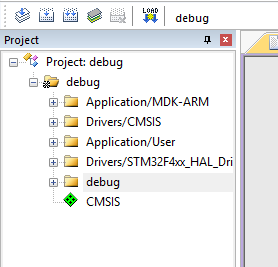
\includegraphics[width=0.6\linewidth]{module.png}
 \caption{Module hóa trong KeilC}
\end{figure}
\paragraph{}
Trong keilC, các file có chức năng tương đương nhau được gộp vào các thư mục.

\paragraph{}
Còn trong Arduino thì hơi củ chuối hơn xíu, bạn phải bỏ toàn bộ file vô cùng thư mục với file .ino. Nếu có rất nhiều file thì nhìn sẽ rối.
\newpage 
\begin{figure}[h!]
\centering
 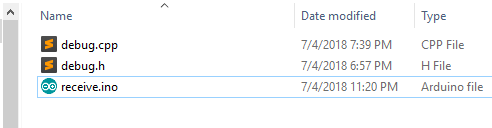
\includegraphics[width=1\linewidth]{arduino_folder.png}
 \caption{Thư mục Arduino}
\end{figure}
\paragraph{}
Nhưng cũng tạm ổn. Và đây là thành quả
\begin{figure}[h!]
\centering
 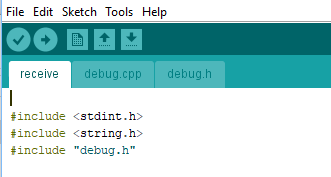
\includegraphics[width=0.8\linewidth]{arduino.png}
 \caption{Module hóa trong Arduino}
\end{figure}
\paragraph{}
Mình từng gặp mấy bạn mới code viết tất cả mọi thứ vào hàm main (kinh dị) từ đọc cảm biến, đọc nút nhấn, điều khiển động cơ... Bạn nên viết hoặc sử dụng thư viện cho mỗi loại phần cứng đó, rồi trong hàm main chỉ gọi hàm trong thư viện đó ra.
\paragraph{}
Nguyên tắc để chia module: module A có thể biết module B làm được \textbf{cái gì} nhưng nó không biết module B làm điều đó \textbf{như thế nào}. Ví dụ bạn sử dụng hàm \textit{Serial.write()} trong Arduino chẳng hạn, bạn biết chắc chắn nó sẽ chuyển dữ liệu đi cho bạn nhưng bạn không cần biết nó chuyển đi như thế nào. A giao việc cho B theo phương thức quy định sẵn và chấm hết. B có thể báo về cho A một số trạng thái như công việc có thành công hay không, hoặc thất bại do nguyên nhân gì.
\paragraph{}
Yêu cầu như trên làm tăng tính độc lập cho các module với nhau, làm cho cả chương trình trở nên rõ ràng hơn. Ví dụ khi lỗi xảy ra, bạn có thể biết được ở A hay B gây ra lỗi, khoanh vùng lỗi nhỏ hơn để dễ kiếm hơn. Khi bạn muốn nâng cấp B để nó chạy nhanh hơn, những chương trình ở A viết sử dụng hàm mà B cung cấp sẽ vẫn hoạt động bình thường, không phải sửa lại mọi thứ. Các thư viện trong Arduino vẫn thường xuyên được cập nhật nhưng chương trình bạn viết vẫn chạy được là vì lí do này.

\section{Cấu trúc chương trình chính và cách gọi hàm}
\paragraph{}
Hàm main trong chương trình chính thường có cấu trúc là khởi tạo và vòng lặp chương trình. 
\begin{lstlisting}
void main(void)
{
	system_init();
	
	while(1)
	{
		//Do what you want
	}
}
\end{lstlisting}
\paragraph{}
Tương tự như arduino nó có setup() và loop().
\begin{lstlisting}
void setup() {
  // put your setup code here, to run once:

}

void loop() {
  // put your main code here, to run repeatedly:

}
\end{lstlisting}
\paragraph{}
Ví dụ như mình viết một chương trình đọc cảm biến và 10 phút gửi về một lần. Thì mình sẽ viết như sau:
\begin{lstlisting}
void main(void)
{
	system_init();
	
	while(1)
	{
		read_sensor();
		send_data();
		delay(10_minutes);
	}
}
\end{lstlisting}
\paragraph{}
Bạn thấy không, chương trình mình viết nó y chang những gì mình nói. Còn việc các hàm đọc cảm biến read\_sensor() hoặc gửi dữ liệu về send\_data() nó ra sao trong đó thì viết ở chỗ khác. Đừng nhét mọi thứ mà bạn có thể viết ra vào đây, làm ơn!!!
\paragraph{}
Có một khái niệm về \textbf{mức trừu tượng}. Ví dụ như hàm đọc cảm biến read\_sensor có thể bao gồm 3 hàm thế này:
\begin{lstlisting}
void read_sensor(void)
{
	request_sensor_data();
	wait_for_sensor_data();
	save_sensor_data();
}
\end{lstlisting}
đầu tiên ra lệnh cho cảm biến, sau đó chờ và khi dữ liệu về thì cất đâu đó. Bạn có thể thấy mức trừu tượng của hàm read\_sensor sẽ cao hơn 3 hàm trong đó vì nó bao hàm 3 cái hàm này. Hàm read\_sensor thì có mức trừu tượng bằng với hàm 2 hàm còn lại trong vòng while(1) của hàm main vì đây là 3 bước tuần tự nhau trong một công việc.
\paragraph{}
Nói tóm lại hãy phân thứ bậc cho các hàm (như mô hình đa cấp ấy :) và khi một hàm gọi các hàm con thì nhớ rằng các hàm con nên có cùng mức trừu tượng với nhau.
\begin{figure}[h!]
	\centering
	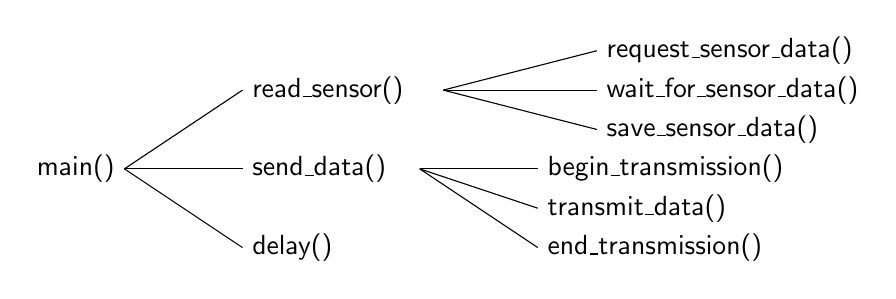
\begin{tikzpicture}[yscale=0.5, xscale=1.5]
	\node [left] at (0, 0) {main()};

	\draw (0,0) -- (1, 2);
	\node [right] at (1,2) {read\_sensor()};
		\draw (2.7,2) -- (4, 3);
		\node [right] at (4,3) {request\_sensor\_data()};
		\draw (2.7,2) -- (4, 2);
		\node [right] at (4,2) {wait\_for\_sensor\_data()};
		\draw (2.7,2) -- (4, 1);
		\node [right] at (4,1) {save\_sensor\_data()};
	\draw (0,0) -- (1, 0);
	\node [right] at (1,0) {send\_data()};
		\draw (2.5,0) -- (3.5, 0);
		\node [right] at (3.5,0) {begin\_transmission()};
		\draw (2.5,0) -- (3.5,-1);
		\node [right] at (3.5, -1) {transmit\_data()};
		\draw (2.5,0) -- (3.5, -2);
		\node [right] at (3.5, -2) {end\_transmission()};

	\draw (0,0) -- (1, -2);
	\node [right] at (1,-2) {delay()};
	
		
	\end{tikzpicture}
	\caption{Mô hình đa cấp.}
\end{figure}
\paragraph{}
Nhớ là hông phải mình làm màu mà viết tên hàm tiếng Anh đâu, vì tiếng Việt không dấu nó như teencode vậy đọc không nổi, mà nhiều khi hiểu lộn nghĩa :).
\section{Hàm số}
\paragraph{}
Việc phát minh ra các hàm con là phát minh vĩ đại như phát minh ra cái máy tính vậy. Nếu không có hàm con thì bạn tưởng tượng viết chương trình một lèo từ đầu tới cuối xem.
\paragraph{}
Vậy nên để đạt hiệu quả thì cần có những lưu ý sau:
\subsection{Đặt tên hàm}
\paragraph{}
Tên hàm được đặt để cho biết cái \textbf{hàm con đó nó làm cái gì}. Ví dụ như read\_sensor() chẳng hạn, dù bạn chưa biết cảm biến loại gì và đọc nó như thế nào nhưng cũng hiểu sơ sơ về mục đích gọi hàm.
\paragraph{}
Và hàm \textbf{nên chỉ thực hiện một chức năng duy nhất}. Nó chỉ làm những gì mà tên hàm nói đến, không hơn không kém. Trong khi viết code thì mọi thứ nên được viết tường minh ra. Ví dụ như hàm gọi hàm send\_data() để truyền dữ liệu về, nếu khi truyền xong muốn xóa dữ liệu cũ đi thì gọi hàm delete\_data() sau khi gọi hàm send\_data().
\begin{lstlisting}
while(1)
{
	read_sensor();
	send_data();
	delete_data();
	delay(10_minutes);
}
\end{lstlisting}
Không nên nhét hàm delete\_data() vào bên trong send\_data() như muốn hiểu ngầm "gửi xong rồi xóa nó đi chứ để làm gì". Vì nhiều khi có việc cần đến nó. Việc viết tường mình, tránh những chỗ hiểu ngầm sẽ giúp người đọc nắm đủ các bước thực hiện của bạn. Hãy viết theo kiểu cho một người chưa biết gì về chương trình của bạn đọc. Và đặc biệt tránh kiểu viết trẻ trâu thích thể hiện, viết đoạn code thật ngầu, thật nhỏ xíu mà vẫn chạy ngon. Sau này chỉ khổ cho mấy người phải đọc lại nó.
\paragraph{}
Hàm được thực thi càng chính xác với cái tên của nó bao nhiêu thì code của bạn sẽ càng dễ đọc bấy nhiêu. 
\paragraph{}
Một vài ví dụ như khi viết vội có bạn đặt tên hàm kiểu ham\_a(), ham\_b(), hoặc func\_1(), func\_2(), mai mốt đọc lại xỉu.
\paragraph{}
Việc bạn đặt tên hàm rồi sau thấy củ chuối quá thì cũng đừng ngại đổi lại, mình nhiều khi cũng phải đổi 2-3 lần mới được cái tên vừa ý.
\subsection{Độ dài của hàm}
\paragraph{}
Nguyên tắc để dễ code dễ đọc: code ngắn thôi, với lại tên hàm đặt đúng với yêu cầu. 
\paragraph{}
Một số hàm chỉ hoạt động tốt nếu nó đủ dài, cắt ngắn lại thành ra dở. Tuy nhiên đa số các trường hợp bạn có thể cắt một hàm dài bất tận ra thành các hàm nhỏ, như chia giai đoạn ra, rồi đặt tên hàm theo các giai đoạn của chương trình. Rất thường xuyên hàm viết ra để gọi có một lần, nó không có tác dụng là tránh lặp lại code như mục đích sinh ra hàm ban đầu, nó chỉ có tác dụng làm chương trình bạn gọn gàng hơn, dễ đọc hơn.
\paragraph{}
Còn độ dài của nó bao nhiêu là vừa. Cái này bạn phải làm rồi rút ra kinh nghiệm cho bản thân. Với mình thì dài dưới 10 dòng là okie nhất, trên 20 dòng thì nên cắt nó đi.
\subsection{Truyền tham số}
\paragraph{}
Tham số là nơi giao tiếp của hàm này với hàm kia. Nó là nơi giao thương nên giống như cái chợ vậy, rất nhiều vấn đề phát sinh. Mà nói chung là một hàm nên hạn chế các tham số đầu vào, chỉ giữ lại nhưng tham số tối quan trọng. Bạn viết một hàm với yêu cầu truyền 5 cái thông số đầu vào thì làm sao bạn nhớ được thứ tự của tham số đó mà truyền cho đúng?
%viet tiep
\subsection{Bảo vệ hàm số}
\paragraph{}
Giả sử bạn viết một hàm chia a cho b như sau:
\begin{lstlisting}
float a_divide_b(int a, int b)
{
	return (float)a/b;
}
\end{lstlisting}

\paragraph{}
Rồi bỗng một ngày đẹp trời, một thanh niên lấy hàm bạn viết ra, rồi xài như sau: \textit{float result = a\_divide\_b(2, 0)}. Xong biên dịch thì không báo lỗi nhưng mà chạy cái nó xịt khói. Đây là lỗi chia cho 0, thành ra nó không tính được và chạy loạn xạ.
\paragraph{}
Thế nên với mỗi chương trình có truyền tham số vào, hãy nhớ là kiểm tra coi nó có hợp lệ hay không, nếu tính toán thì tham số đưa vào có thuộc tập xác định hay không... Bởi vì bạn sẽ không biết sau này người dùng hàm sẽ truyền cái gì vào trong đó nên phải kiểm tra lại. Nguyên tắc kiểm tra là : không tin cha con thằng nào cả. Đừng hi vọng họ sẽ truyền vào tham số hợp lệ, thường thì họ chả quan tâm đâu. Nên nhớ kiểm tra đầu vào hợp lệ thì mới thực thi hàm.
\paragraph{}
Hàm có kiểm tra tham số đầu vào:
\begin{lstlisting}
float a_divide_b(int a, int b)
{
	if(b==0){
		//printf("Divided by 0 error\n");
		return 0;
	}
	return (float)a/b;
}
\end{lstlisting}

\section{Các biến số}
\paragraph{}
Tất nhiên là khi lập trình bạn đều phải khai báo biến, rồi sử dụng các biến đó để lưu trữ, tính toán. Thế nên việc sử dụng cẩn thận các biến là điều rất quan trọng để chương trình có thể chạy được và ít phát sinh lỗi.
\subsection{Đặt tên biến}
\paragraph{}
Cũng giống như việc đặt tên hàm, một biến được đặt tên để biến nó sinh ra để làm cái gì. Bạn có thể thấy cách mà mình đặt tên cho kiểu \textit{env\_t}, bao gồm \textit{temp, humi, lux}, nếu bạn sử dụng quen thì có thể biết từng biến trong đó lưu giá trị gì mà không bị nhầm lẫn (viết tắt của temperature, humidity, lux). Có nhiều bạn sử dụng các chữ cái như a, b, c... hoặc x1, x2 để đặt tên biến, nhưng mà tin mình đi, mấy cái đó đọc nhức mắt kinh khủng, đôi khi trong lúc code bạn cũng không nhớ khai báo nó để lưu cái gì nữa. Tại hại hơn là bạn lại lưu vào x1 giá trị đáng lí ra phải lưu vào x2.
\paragraph{}
Theo thói quen thì cái chữ cái như i, j... được dùng trong vòng lặp cho tiện. Điều này cũng không có vấn đề gì nhiều nếu bạn sử dụng quen nó.
\subsection{Các lưu ý khi khai báo biến}
\paragraph{}
Khi khai báo và sử dụng biến nên chú ý những điểm sau:
\begin{itemize}
\item Tránh sử dụng biến toàn cục (global variable): biến toàn cục được khai báo bên ngoài hàm, là nơi mà bất kì hàm nào cũng có thể truy cập và chỉnh sửa nó. 
\begin{lstlisting}
int a; //this is a global variable

void setup(){
}

void loop(){
}
\end{lstlisting}
\paragraph{}
Hãy tưởng tượng là trong file này của bạn có khoảng 20 hàm được khai báo, mà hàm nào cũng có quyền truy cập vào biến toàn cục này, nên bất cứ lúc nào nó cũng có thể bị thay đổi. Tệ hơn nữa nếu không phải do một mình bạn viết mà do vài người viết nên file code này, việc không hiểu rõ ý mà tự tiện truy cập vào biến toàn cục là chuyện bình thường.
\paragraph{}
Thế nên hãy hạn chế biến toàn cục hết mức có thể, và tốt nhất là không khai báo biến kiểu này càng tốt. Khi nhất thiết phải sử dụng biến toàn cục thì nên chú thích rõ những nơi nào được đọc, ghi biến này để tránh việc thay đổi biến mà không biết trước.
\paragraph{}
Biến toàn cục là đồ công cộng. Ai cũng đụng chạm nó được. Mà đồ công cộng thì không an toàn. Thế thôi.
\item Hãy khởi tạo giá trị cho biến: Thay vì khai báo \textit{int a;} thì hãy khai báo \textit{int a=0;}. Đôi khi việc bạn khai báo biến thì CPU chỉ định vị biến này trong bộ nhớ mà không tự khởi tạo biến này với giá trị mặc định là 0 có thể gây lỗi, nhất là ngay sau đó bạn dùng phép toán \textit{or} chẳng hạn.
\item Luôn chắc rằng biến của bạn có thể chứa đủ giá trị mà bạn muốn lưu vào trong đó. Ví dụ như việc sử dụng biến uint8\_t, với khoảng giá trị từ 0 tới 255, nếu tình cờ mà bạn ghi vào con số lớn hơn khoảng giá trị này thì nó sẽ xịt khói lập tức.
\end{itemize}
\subsection{Kiểu biến static}
\subsection{Kiểu biến \textit{volatile}}

\section{Chú thích}
\paragraph{}
Chú thích (comment) tưởng đơn giản nhưng lại là thành phần hại não trong khi viết chương trình. Bạn có thể thấy trong C thì chú thích đi sau dấu // hoặc /* */. Tại sao nó hại não? Vì nếu chú thích đúng cách thì chương trình rất dễ đọc và người khác (ngay cả bạn nữa) cũng nắm được đại ý nhanh chóng. Nhưng khổ cái là chương trình thay đổi liên tục, mà hễ thay đổi thì chỉnh sửa code lại thôi, không ai chịu sửa lại chú thích làm chi (vì sửa code không cũng đuối rồi). Nên làm cho người đọc tưởng là mình hiểu rồi nhưng một hồi đọc tới code thì thấy nó sai sai.
\paragraph{}
Thế nên cách chú thích tốt nhất là hạn chế nó hết mức có thể. Sử dụng tên hàm, tên biến như là một loại chú thích hiệu quả hơn.
\paragraph{}
Tất nhiên là bạn không nên bỏ hẳn nó đi, vì nếu sử dụng nó đúng cách thì nó đem lại hiệu quả rất nhiều. Các chương trình thường đặt chú thích lên đầu trang để giải thích khái quát coi chương trình đó đùng để làm gì. Trong file \textit{.h}, các chú thích được đặt trước tên hàm giải thích công dụng của hàm đó, để người sử dụng có thể sử dụng luôn thư viện mà không cần phải đọc tới file code. Đôi khi những đoạn code khó đọc, tính logic cao thì nên có chú thích để giải thích coi ý tưởng đằng sau đoạn code đó là gì, nó giải quyết vấn đề gì.

\section{Blocking vs. Non-blocking mode}
\paragraph{}
Blocking là gì? Hãy xem qua chương trình chớp tắt led trong Arduino như sau:
\begin{lstlisting}
void loop() {
  digitalWrite(LED_BUILTIN, HIGH);   // turn the LED on (HIGH is the voltage level)
  delay(1000);                       // wait for a second
  digitalWrite(LED_BUILTIN, LOW);    // turn the LED off by making the voltage LOW
  delay(1000);                       // wait for a second
}
\end{lstlisting}
\paragraph{}
Có thể thấy là nó bật led, sử dụng hàm delay() trong 1 giây rồi tắt led, tiếp tục delay() và chương trình lặp lại liên tục.
\paragraph{}
Vấn đề là ở chỗ hàm delay(), chương trình đứng yên một chỗ và không làm gì cả, hay nói cách khác là nó bị \textbf{block} tại chỗ đó. Viết chương trình có chứa hàm tạm dừng một chỗ như delay() thì người ta gọi là \textbf{Blocking mode}. Trong thế giới nhúng, tài nguyên hạn chế nên chương trình đứng một chỗ như vậy là việc hết sức lãng phí. Thế nên có kiểu viết khác gọi là \textbf{Non-Blocking mode} nhằm làm cho chương trình chạy liên tục mà không bị đứng tại một điểm nào cả.
\paragraph{}
Ví dụ về viết kiểu Non-blocking cho chương trình chớp tắt led. Ý tưởng đằng sau này là lưu lại thời gian của lần bật/tắt led lần trước, rồi so sánh với thời điểm hiện tại, nếu nó vượt quá 1 giây chẳng hạn, thì tiến hành lần bật tắt tiếp theo.
\begin{lstlisting}
void loop() {
static uint32_t last_action;
  if(millis()-last_action>1000)
  {
    toggle_led(LED_BUILTIN);
    last_action_millis=millis();
  }
}
\end{lstlisting}
\paragraph{}
Như đoạn code trên, last\_action lưu lại thời gian của hoạt động bật/tắt led lần trước, lưu ý là nó phải được khai báo \textit{static} để không khởi tạo lại khi vòng loop bắt đầu vòng lặp mới. Và cả chương trình sẽ được viết như sau: 
\begin{lstlisting}
void setup() {
  // initialize digital pin LED_BUILTIN as an output.
  pinMode(LED_BUILTIN, OUTPUT);
}

void toggle_led(uint8_t led)
{
  uint8_t led_state=digitalRead(led);
  if(led_state==HIGH)
    digitalWrite(led, LOW);
  else
    digitalWrite(led, HIGH);
}

// the loop function runs over and over again forever
void loop() {
static uint32_t last_action;
  if(millis()-last_action>1000)
  {
    toggle_led(LED_BUILTIN);
    last_action=millis();
  }
}
\end{lstlisting}
\paragraph{}
Với cách viết như trên thì chương trình không bị đứng ở bất cứ điểm nào. Trong hàm loop(), chương trình liên tục hỏi đã đến lúc bật/tắt led hay chưa, nếu đến lúc thì thực hiện bật/tắt và lưu lại thời điểm vừa thực hiện. Nếu chưa thì thoát xuống làm chuyện khác. Đến đây bạn có thể viết chương trình điều khiển 2 led như sau:

\begin{lstlisting}

void control_led_1(){
  static uint32_t last_action;
  if(millis()-last_action>1000)
  {
    toggle_led(led_1);
    last_action=millis();
  }	
}

void control_led_2(){
  static uint32_t last_action;
  if(millis()-last_action>1000)
  {
    toggle_led(led_2);
    last_action=millis();
  }	
}

void loop() {
	control_led_1();
	control_led_2();
}
\end{lstlisting}
\paragraph{}
Rồi đến đây thì bạn vừa có thể tiết kiệm được tài nguyên CPU, bằng cách làm nhiều tác vụ tuần tự nhau, vừa có thể thêm một số tính năng mới mà không cần phải đập đi xây lại, sugoi!!! Nhớ là mỗi tính năng bạn thêm vào đều phải đảm bảo tính Non-blocking he.
\section{Máy trạng thái}
\paragraph{}
Máy trạng thái (state machine) là thứ rất thường gặp trong lập trình nhúng. Ví dụ bạn viết chương trình điều khiển một cái động cơ, thì nó sẽ có những trạng thái như là đang dừng, đang quay ngược chiều hoặc cùng chiều kim đồng hồ... Máy trạng thái có thể hiểu là sơ đồ tất cả các trạng thái của một đối tượng nào đó và những điều kiện để chuyển từ trạng thái này sang trạng thái khác. Dưới đây là một ví dụ về chớp tắt led.
\begin{figure}[h!]
	\centering
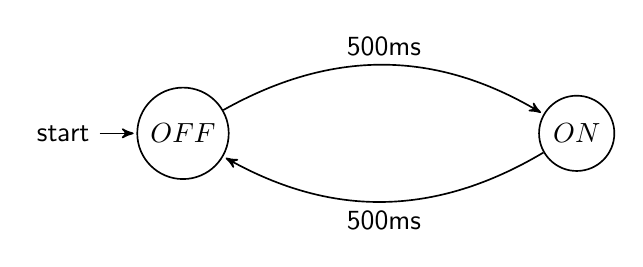
\begin{tikzpicture}[->,>=stealth',shorten >=1pt,auto,node distance=5cm,
                    semithick]

  \node[initial,state] (A)                    	{$OFF$};
  \node[state]         (B) [right of=A] 		{$ON$};

  \path (A) edge [bend left]            node {500ms} (B)
        (B) edge [bend left]            node {500ms} (A);
 
\end{tikzpicture}
\caption{Chớp tắt led.}
\end{figure}
\paragraph{}
Đầu tiên bạn có thể thấy nó sẽ tắt led, và sau mỗi nửa giây nó lại đổi trạng thái một lần.
\paragraph{}
Các bạn có thể tham khảo về sơ đồ máy trạng thái kĩ hơn ở cuốn sách này \textit{\url{http://nxbdhqghcm.edu.vn/san-pham/1/sach/30/bia-quyet-lam-dep/1099/lap-trinh-he-thong-nhung.htm}}. Do trong đấy nói chi tiết nên mình sẽ không lặp lại nữa (do ông viết sách là sư phụ mình nên quảng cáo xíu :)).
\begin{comment}
\section{Lưu đồ giải thuật}

\paragraph{}
Có bạn nào viết lưu đồ giải thuật (flowchart) ra rồi mới code không, hay toàn làm ngược lại, code rồi mới viết lưu đồ ra cho có rồi đem nộp?
\paragraph{}
Lưu đồ giải thuật thường viết khi bạn thực hiện một đoạn chương trình khó, nặng tính logic. Còn thông thường thì không cần nó làm chi. Hồi sinh viên viết mấy đoạn dễ ẹc nên không bao giờ mình viết lưu đồ ra, có viết thì để làm báo cáo thôi. Giờ đi làm gặp những thứ chua ăn hơn, nếu không viết nó ra thì không biết code thế nào cho đúng. 
\paragraph{}
Và lưu đồ giải thuật sẽ tập cho bạn thói quen suy nghĩ trước khi làm, chứ không phải là làm theo cảm tính rồi ngồi sửa. Hãy nhớ code chỉ là một phần của sản phẩm bạn tạo ra, hãy dành thời gian suy nghĩ về cấu trúc của sản phẩm, thiết kế từng module rồi vẽ lưu đồ nếu cần. Đó là bước bạn làm cho ý tưởng của bạn nó rõ ràng, cách diễn đạt được mạch lạc. Cuối cùng là chỉ cho cái máy hiểu bạn muốn nó làm cái chi (là viết chương trình đó). Đừng cắm đầu code khi bạn còn chưa biết bạn sẽ làm cái gì nữa.
\paragraph{}
Rồi một ví dụ về bên nhận dữ liệu uart (lại là uart). Bên nhận thì nhìn chung không biết thằng phát sẽ phát bao nhiêu, nó không biết bao giờ sẽ kết thúc cái chuỗi mà nó đang nhận. Vậy làm thế nào để khi bên phát hết phát thì bên thu sẽ biết mà còn đi làm cái khác?
\paragraph{}
Có rất nhiều cách. Như người ta có thể chuyển dữ liệu sang chỗi json (đại khái toàn là chuỗi kí tự mã ASCII và dữ liệu không bao giờ có kí tự kết thúc chuỗi '\textbackslash0') và sau đó thêm kí tự '\textbackslash0' vào cuối chuỗi, bên nhận nhận được kí tự này và báo về chương trình chính đã nhận xong. Nhưng ở đây mình sử dụng cách đơn giản hơn, nếu nó đang nhận dữ liệu và đột nhiên không nhận được nữa trong vòng 20 mili giây thì nó sẽ báo là nhận xong rồi.
\paragraph{}
Rồi viết ra yêu cầu của chương trình rồi giờ tới thiết kế. Bạn tự làm thử xem :)))
\paragraph{}
Theo yêu cầu thì bộ truyền nhận sẽ có 2 trạng thái: WAITING (đang chờ dữ liệu, kí hiệu WAIT=0) và RECEIVING (đang nhận, kí hiệu RECV=1). Khi mới khởi tạo thì nó sẽ có trạng thái đang chờ. Khi nhận được thông báo có dữ liệu đến thì nó sẽ chuyển qua trạng thái đang nhận. Nhận xong thì trở về WAITING.
\begin{figure}[h!]
	\centering
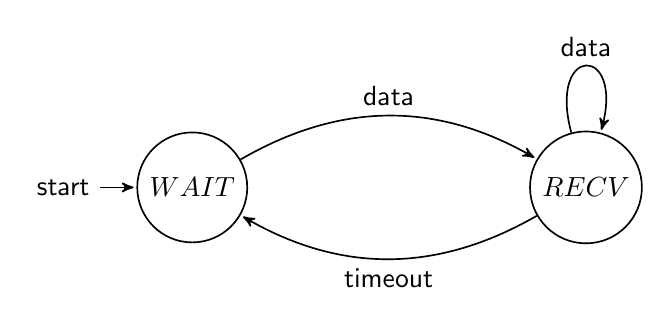
\begin{tikzpicture}[->,>=stealth',shorten >=1pt,auto,node distance=5cm,
                    semithick]

  \node[initial,state] (A)                    	{$WAIT$};
  \node[state]         (B) [right of=A] 		{$RECV$};

  \path (A) edge [bend left]            node {data} (B)
        (B) edge [loop above] 			node {data} (B)
            edge [bend left]            node {timeout} (A);
 
\end{tikzpicture}
\caption{Lưu đồ máy trạng thái.}

\end{figure}
\paragraph{}
Trên là lưu đồ đơn giản nhất. Trong chương trình mình sẽ viết theo kiểu non-blocking, tức là không có sử dụng hàm delay() mà chương trình sẽ liên tục kiểm tra ngõ vào. Tài nguyên có hạn nên bạn không nên phung phí nó mà sử dụng hàm delay(), chương trình sẽ đứng nguyên một chỗ. Có thời gian thì mình sẽ viết chi tiết hơn.
\paragraph{}
Rồi giờ tới lưu đồ cho anh kia.
\begin{figure}
\centering
\begin{tikzpicture}[node distance=2cm]

\node (start) [startstop] {Begin};
\node (dec1) [decision, below of=start, yshift=-0.5cm] {state=0?};
\draw [arrow] (start) -- (dec1);

\node (dec2) [decision, left of=dec1, xshift=-1cm] {data?};
\draw [arrow] (dec1) -- node [above] {Y} (dec2);

\node (dec3) [decision, right of=dec1, xshift=1cm] {data?};
\draw [arrow] (dec1) -- node [above] {N} (dec3);

\node (pro1) [process, right of=dec3, xshift=1cm] {get data?};
\draw [arrow] (dec3) -- node [above] {Y} (pro1);
\node (dec4) [decision, below of=dec3, yshift=-0.5cm] {timeout?};
\draw [arrow] (dec3) -- node [right] {N} (dec4);


\node (stop) [startstop, below of=start, yshift=-10cm ] {End};
\draw [arrow] (pro1) |-  (stop);
%\node (pro2a) [process, below of=dec1, yshift=-0.5cm] {Process 2a};
%\node (stop) [startstop, below of=out1] {Stop};
%\draw [arrow] (start) -- node [right] (dec1);

\end{tikzpicture}
\caption{Lưu đồ giải thuật.}
\end{figure}


\paragraph{}
\end{comment}

\chapter{Viết thư viện}
\paragraph{}
Nếu bạn đi theo con đường lập trình chuyên nghiệp thì bạn phải chuẩn bị cho mình một bộ thư viện để khi cần thì có thể lôi ra sử dụng. Trên Arduino được hỗ trợ rất nhiều nhưng không có nghĩ là đúng và  đủ. Tất cả thư viện đó đều có thể có lỗi và đôi khi có những thư viện chưa được hỗ trợ. Hoặc trường hợp thường gặp như thư viện của cảm biến DHT11 đã có trên Arduino nhưng dự án của bạn lại sử dụng chip khác thì cần biết làm sao để chuyển từ thư viện Arduino sang loại chip mà bạn đang sử dụng.
\paragraph{}
Trên Arduino thư viện được viết bằng C++ nhưng mà mình sẽ hướng dẫn bạn viết bằng C, vì nó dễ hơn. Sau này rành rồi thì bạn cũng nên tự học C++ vì nó có nhiều chiêu hay hơn C (nó hơn hai đấu cộng lận đó).
\section{Cấu trúc thư viện}
\paragraph{}
Một thư viện có thể có rất nhiều file trong đó. Nhưng cơ bản thì nó có 2 file chính: file code \textit{.c} và file header \textit{.h}. File code thì tất nhiên là để viết code rồi. Nhưng mà có ai sử dụng thư viện mà lôi code ra đọc từ đầu đến cuối rồi mới sử dụng đâu. Đó là lí do sinh ra file \textit{.h}. Nó là nơi \textbf{khai báo hàm}, bao gồm các hàm mà trong thư viện mà bạn có thể xài, các cấu trúc dữ liệu... và đặc biệt là phải có các đoạn hướng dẫn sử dụng, để người dùng chỉ cần đọc hướng dẫn thôi là sử dụng được cái thư viện đó rồi. Cho nên thư viện của bạn viết, ngoài đáp ứng 3 tiêu chí chạy được, dễ thay đổi, dễ hiểu ra, còn thêm một yêu cầu cho thư viện là dễ sử dụng nữa.
\paragraph{}
Đối với Arduino thì bạn cần đặt 2 file này vào cùng thư mục của với file .ino, còn như sử dụng các chip khác thì mỗi thư viện cần có một thư mục riêng.
\paragraph{}
Một ví dụ về thư viện:
\begin{lstlisting}
//file example.h
#ifndef _EXAMPLE_H
	#define _EXAMPLE_H

	//Initiate example library 
	void example_init(void);

	//Example function
	void example_function(void);

#endif
\end{lstlisting}

\begin{lstlisting}
//file example.c
#include "example.h"

void example_init(void){
	//do something
}

void example_function(void){
	//do something
}

\end{lstlisting}

\paragraph{}
Lưu ý: đoạn macro
\begin{lstlisting}
//file example.h
#ifndef _EXAMPLE_H
	#define _EXAMPLE_H
	.
	.
	.
#endif
\end{lstlisting}
Là rất quan trọng, mỗi file \textit{.h} nên có một đoạn này, và \_EXAMPLE\_H thay đổi tùy theo tên hàm của bạn.
\paragraph{}
Có thể giải thích như sau: trong C nó có một bộ tiền xử lý (preprocessor), là trước khi biên dịch code của bạn thì nó sẽ làm việc của cái bộ tiền xử lý này trước. Cặp khai báo \#ifndef \#endif sẽ đi chung với nhau. Đoạn khai báo trên có nghĩa là: Nếu chưa định nghĩa \_EXAMPLE\_H thì định nghĩa \_EXAMPLE\_H và mấy cái bên dưới, cho tới chỗ \#endif thì dừng.
\paragraph{}
Giả sử mình có file a.h , b.h được khai báo như sau:

\begin{lstlisting}
//file a.h
int A=0;
\end{lstlisting}
\begin{lstlisting}
//file b.h
#include "a.h"
int B=0;
\end{lstlisting}
và có thêm một file c.h
\begin{lstlisting}
//file c.h
#include "a.h"
#include "b.h"
int C=0;
\end{lstlisting}
bạn có thể thấy, khi c \textit{\#include "a.h"} thì nó đã khai báo một biến A trong đó rồi. Khi c \textit{\#include "b.h"} thì nó khai báo tiếp 2 biến A, B nữa, vậy biến A được khai báo 2 lần và sẽ gây lỗi.
\paragraph{}
Tất nhiên là bạn không nên khai báo biến trong file \textit{.h}, nhưng ở đây là ví dụ về trường hợp sẽ sinh ra lỗi. Nếu sử dụng cặp khai báo  \#ifndef \#endif thì sẽ giải quyết được chuyện này. 
\begin{lstlisting}
//file a.h
#ifndef _A_H
	#define _A_H
	int A=0;
#endif
\end{lstlisting}
\begin{lstlisting}
//file b.h
#ifndef _B_H
	#define _B_H
	#include "a.h"
	int B=0;
#endif
\end{lstlisting}

khi c \textit{\#include "a.h"} thì nó sẽ khai báo biến A và định nghĩa chuỗi \_A\_H (định nghĩa này là ghi nhận nó đã từng xuất hiện trên đời). Khi c \textit{\#include "b.h"}, thì đầu tiên b.h sẽ  \textit{\#include "a.h"}, nhưng nó thấy \_A\_H đã từng xuất hiện rồi nên không khai báo phần bên dưới nữa. Rồi cuối cùng nó chỉ định khai báo biến B thôi.
\paragraph{}
Tóm lại là đoạn macro đó giúp bạn không bị khai báo lại khi mà \textit{\#include} chồng chéo nhiều thư viện khác nhau.
\paragraph{}
Một lưu ý khác là thư viện C của bạn có thể được sử dụng bởi một chương trình C++, nên cách viết để C++ có thể đọc nó như sau:
\begin{lstlisting}
//file example.h
#ifndef _EXAMPLE_H
	#define _EXAMPLE_H
	
	#ifdef __cplusplus
 		extern "C" {
	#endif

	//Initiate example library 
	void example_init(void);

	//Example function
	void example_function(void);
	
	#ifdef __cplusplus
	}
	#endif
	
#endif
\end{lstlisting}
hãy làm quen với bộ tiền xử lý vì nó được sử dụng nhiều lắm.
\section{Viết thư viện theo phong cách OOP}
\paragraph{}
Rồi, sau khi bạn có thói quen chia chương trình thành cách file thư viện nhỏ rồi, không còn nhét mọi thư vôi main.c nữa thì bạn có thể đến bước này.
\paragraph{}
Lập trình hướng đối tượng (OOP) là một bước tiến của lập trình cấu trúc ( ngôn ngữ C là hướng cấu trúc, C++ là hướng đối tượng). OOP có nhiều ưu điểm hơn, sử dụng được cho những chương trình lớn hơn. C không phải là ngôn ngữ hướng đối tượng nhưng bạn có thể bắt chước phong cách OOP và cuộc sống sẽ dễ dàng hơn.
\paragraph{}
Bạn hoàn toàn có thể sử dụng C++ cho Arduino nhưng các chip khác thường vẫn sử dụng C, và bạn làm việc với C một thời gian mà chuyển lên C++ mới thấy nó rất phê, giống như chuyển từ assemply qua C vậy. Còn mà xài C++ ngay từ đầu luôn thì nó cũng thường thôi.
\paragraph{}
Vào vấn đề chính. Mình muốn viến thư viện điều khiển một cái relay (rờ le). Bình thường thì nó tắt. Khi nào bạn muốn bật nó lên thì ngoài gọi lệnh như turn\_relay\_on() ra bạn còn phải truyền thời gian khi nào nó tắt nữa, không để nó chạy hoài, vì nhiều khi relay đang kéo tải công suất lớn như máy bơm hay đèn gì đấy. Và tất nhiên là có thể dừng nó bất kì lúc nào và điều khiển một lúc nhiều relay khác nhau.
\paragraph{}
Trước tiên là khai báo một struct cho mỗi relay:
\begin{lstlisting}
//relay.h

//low active or high active
#define ON HIGH
#define OFF LOW
typedef struct{
	uint8_t pin;
	uint8_t state;
	uint32_t on_state_begin;
	uint32_t on_state_timeout;
}relay_t;
\end{lstlisting}
\textit{pin} là xem relay đó nối với chân nào của Arduino, state là trạng thái nó đang ON hay OFF, \textit{on\_state\_begin} là thời điểm bắt đầu ON, còn \textit{on\_state\_timeout} là thời gian ON của nó, hết cái đó nó sẽ tắt.
\paragraph{}
Sau đó sẽ khai báo các hàm sử dụng struct này:
\begin{lstlisting}
//relay.h
//initiate relay first
void relay_init(relay_t *relay, uint8_t pin);
void turn_relay_on(relay_t *relay, uint32_t timeout);
void turn_relay_off(relay_t *relay);
//return true if relay high state timeout
bool is_relay_on_state_timeout(relay_t *relay);
\end{lstlisting}
\paragraph{}
Và rồi trong chương trình chính mình sẽ sử dụng nó như sau.
\begin{lstlisting}

#include "relay.h"

relay_t relay;

void setup(){
	relay_init(&relay, 5); //pin 5 control this relay
	delay(1000);
	turn_relay_on(&relay, 1000);
}

void loop(){
	if(is_relay_on_state_timeout(&relay)){
		turn_relay_off(&relay);
	}
}

\end{lstlisting}
\paragraph{}
Chương trình chính ở setup() sẽ bật relay đó lên và trong loop() liên tục hỏi coi nó có timeout chưa, nếu có thì tắt relay đó đi. Lưu ý là hàm is\_relay\_on\_state\_timeout() chỉ trả về true nếu relay đó đang ON và đã hết thời gian, trả về false nếu đang OFF hoặc chưa timeout.
\paragraph{}
Bạn hoàn toàn có thể khai báo một mảng relay\_t relay[8] để điều khiển một lúc 8 cái relay. Mỗi cái cần một lần khởi tạo và gắn chân riêng, con trỏ truyền vào có thể là \&relay[0] để điều khiển relay số 0.
\paragraph{}
Cái tinh thần của OOP trong đây là bạn khai báo một biến (coi nó như một đối tượng), rồi sau đó không động chạm gì đến thành phần bên trong của biến đó mà chỉ sử dụng các hàm được khai báo sẵn để tương tác với biến đó. Các thành phần bên trong biến sẽ được truy cập tại thư viện. 
\paragraph{}
Viết thư viện theo kiểu này sẽ đảm bảo bao đóng của dữ liệu để đối tượng nó được an toàn. Như bạn thấy biến state trong kiểu relay\_t là một biến nội bộ lưu lại trạng thái của relay. Như hàm turn\_relay\_on() sẽ có lệnh digitalWrite(pin, ON) và gán biến state=ON bên trong. Nếu bạn tự tiện gán relay.state=OFF trong chương trình chính thì sẽ bị lỗi (xem code bên dưới).
\paragraph{}
Việc bao đóng dữ liệu sẽ giúp các module độc lập hơn. Bạn không cần quan tâm trong biến relay\_t có cái gì ở trỏng. Chỉ cần khai báo, rồi gọi hàm truyền nó vào. Như vậy nó đảm bảo được nguyên tắc A biết B làm được cái gì chứ không biết B làm điều đó như thế nào.

\paragraph{}
Sau đây là phần code cho relay đó:
\begin{lstlisting}
//relay.c
void relay_init(relay_t *relay, uint8_t pin)
{
	relay->pin=pin;
	pinMode(relay->pin, OUTPUT);
	digitalWrite(relay->pin, OFF);
	relay->state=OFF
}

void turn_relay_on(relay_t *relay, uint32_t timeout)
{
	digitalWrite(relay->pin, ON);
	relay->state=ON;
	relay->on_state_begin=millis();
	relay->on_state_timeout=timeout;
}

void turn_relay_off(relay_t *relay)
{
	digitalWrite(relay->pin, OFF);
	relay->state=OFF;
}

bool is_relay_on_state_timeout(relay_t *relay)
{
	if(relay->state==ON) 
	{
		if((millis() - relay->on_state_begin)\
						 > relay->on_state_timeout)
			return true; //return and exit
	}
	return false;
}

\end{lstlisting}
\paragraph{}
Tất nhiên là mình viết sơ sơ để các bạn dễ đọc thôi, còn nhiều cái khác để làm cho thư viện này chạy ổn. Như kiểu người ta chưa init nó lên mà đã gọi hàm ON OFF thì phải làm sao? Haha, tới đây bạn sẽ phát hiện là trong relay.c sửa tá lả làm bên trong chương trình chính không sửa gì vẫn chạy được. Bạn có thể không cần phải điều khiển relay thật luôn mà nháp trước với một con led cũng được.
\paragraph{}
Hãy nghiên cứu phần này để cuộc sống nó dễ chịu hơn.
\chapter{Quản lý phiên bản: GIT}


\end{document}
